%\documentclass[10pt]{article}
%\usepackage[pdftex]{graphicx}
%%$Id: macro.tex,v 1.10 2004/12/08 13:38:58 acary Exp $


%\usepackage{a4wide}
\textheight 25cm
\textwidth 16.5cm
\topmargin -1cm
%\evensidemargin 0cm
\oddsidemargin 0cm
\evensidemargin0cm
\usepackage{layout}


\usepackage{amsmath}
\usepackage{amssymb}
\usepackage{minitoc}
%\usepackage{glosstex}
\usepackage{colortbl}
\usepackage{hhline}
\usepackage{longtable}

%\usepackage{glosstex}
%\def\glossaryname{Glossary of Notation}
\def\listacronymname{Acronyms}

\usepackage[outerbars]{changebar}\setcounter{changebargrey}{20}
%\glxitemorderdefault{acr}{l}

%\usepackage{color}
\usepackage{graphicx,epsfig}
\graphicspath{{./Figures/}}
\usepackage[T1]{fontenc}
\usepackage{rotating}

%\usepackage{algorithmic}
%\usepackage{algorithm}
\usepackage{ntheorem}
\usepackage{natbib}


%\renewcommand{\baselinestretch}{2.0}
\setcounter{tocdepth}{2}     % Dans la table des matieres
\setcounter{secnumdepth}{3}  % Avec un numero.



\newtheorem{definition}{Definition}
\newtheorem{lemma}{Lemma}
\newtheorem{claim}{Claim}
\newtheorem{remark}{Remark}
\newtheorem{assumption}{Assumption}
\newtheorem{example}{Example}
\newtheorem{conjecture}{Conjecture}
\newtheorem{corollary}{Corollary}
\newtheorem{OP}{OP}
\newtheorem{problem}{Problem}
\newtheorem{theorem}{Theorem}


\newcommand{\CC}{\mbox{\rm $~\vrule height6.6pt width0.5pt depth0.25pt\!\!$C}}
\newcommand{\ZZ}{\mbox{\rm \lower0.3pt\hbox{$\angle\!\!\!$}Z}}
\newcommand{\RR}{\mbox{\rm $I\!\!R$}}
\newcommand{\NN}{\mbox{\rm $I\!\!N$}}

\newcommand{\Mnn}{\mathcal M^{n\times n}}
\newcommand{\Mnp}[2]{\ensuremath{\mathcal M^{#1\times #2}}}



\newcommand{\Frac}[2]{\displaystyle \frac{#1}{#2}}

\newcommand{\DP}[2]{\displaystyle \frac{\partial {#1}}{\partial {#2}}}

% c++ variables writting
\newcommand{\varcpp}[1]{\textit{#1}}
% itemize
\newcommand{\bei}{\begin{itemize}}
\newcommand{\ei}{\end{itemize}}

\newcommand{\ie}{i.e.}
\newcommand{\eg}{e.g.}
\newcommand{\cf}{c.f.}
\newcommand{\putidx}[1]{\index{#1}\textit{#1}}

\def\Er{{\rm I\! R}}
\def\En{{\rm I\! N}} 
\def\Ec{{\rm I\! C}}
 
\def\zc{\hat{z}}
\def\wc{\hat{w}}

\font\tete=cmr8 at 8 pt
\font\titre= cmr12 at 20 pt 
\font\titregras=cmbx12 at 20 pt

%----------------------------------------------------------------------
%                  Modification des subsubsections
%----------------------------------------------------------------------
\makeatletter
\renewcommand\thesubsubsection{\thesubsection.\@alph\c@subsubsection}
\makeatother

%----------------------------------------------------------------------
%             Redaction note environnement
%----------------------------------------------------------------------
\makeatletter
\theoremheaderfont{\scshape}
\theoremstyle{marginbreak}
\theorembodyfont{\upshape}
%\newtheorem{rque}{\bf Remarque}[chapter]
%\newtheorem{rque1}{\bf \fsc{Remarque}}[chapter] !!! \fsc est une commande french
\newtheorem{ndr1}{\textbf{\textsc{Redaction note}}}[section]

\newenvironment{ndr}%
{%
\tt
%\centerline{---oOo---}
\noindent\begin{ndr1}%
}%
{%
\begin{flushright}%
%\vspace{-1.5em}\ding{111}
\end{flushright}%
\end{ndr1}%
%\centerline{---oOo---}
}

\makeatother

%----------------------------------------------------------------------
%             Redaction note environnement V.ACARY
%----------------------------------------------------------------------
\makeatletter
\theoremheaderfont{\scshape}
\theoremstyle{marginbreak}
\theorembodyfont{\upshape}
%\newtheorem{rque}{\bf Remarque}[chapter]
%\newtheorem{rque1}{\bf \fsc{Remarque}}[chapter] !!! \fsc est une commande french
\newtheorem{ndr1va}{\textbf{\textsc{Redaction note V. ACARY}}}[section]

\newenvironment{ndrva}%
{%
\tt
%\centerline{---oOo---}
\noindent\begin{ndr1va}%
}%
{%
\begin{flushright}%
%\vspace{-1.5em}\ding{111}
\end{flushright}%
\end{ndr1va}%
%\centerline{---oOo---}
}

\makeatother
%----------------------------------------------------------------------
%             Redaction note environnement V.ACARY
%----------------------------------------------------------------------
\makeatletter
\theoremheaderfont{\scshape}
\theoremstyle{marginbreak}
\theorembodyfont{\upshape}
%\newtheorem{rque}{\bf Remarque}[chapter]
%\newtheorem{rque1}{\bf \fsc{Remarque}}[chapter] !!! \fsc est une commande french
\newtheorem{ndr1fp}{\textbf{\textsc{Redaction note F. PERIGNON}}}[section]

\newenvironment{ndrfp}%
{%
\tt
%\centerline{---oOo---}
\noindent\begin{ndr1fp}%
}%
{%
\begin{flushright}%
%\vspace{-1.5em}\ding{111}
\end{flushright}%
\end{ndr1fp}%
%\centerline{---oOo---}
}

\makeatother
%----------------------------------------------------------------------
%                  Chapter head enviroment
%----------------------------------------------------------------------
\newenvironment{chapter_head}
{%
\begin{center}%
-------------------- oOo --------------------\\%
\ \\%
\begin{minipage}[]{14cm}%
\noindent\normalsize\advance\baselineskip-1pt %
}%
{%
\par\end{minipage}%
\ \\%
\ \\%
-------------------- oOo --------------------
\end{center}%
\vspace*{\stretch{1}}%
\clearpage%
\thispagestyle{empty}%
\vspace*{\stretch{1}}%
\minitoc%
\vspace*{\stretch{2}}%
\clearpage%
}

%%% Local Variables: 
%%% mode: latex
%%% TeX-master: "report"
%%% End: 

%\usepackage{psfrag}
%\usepackage{fancyhdr}
%\usepackage{subfigure}
%\usepackage{layout}
%\usepackage{mathpple}
%\usepackage{color}
%\usepackage{texdraw} % TeXdraw commands
%\renewcommand{\baselinestretch}{1.2}
%\textheight 23cm \textwidth 16cm \topmargin 0cm \evensidemargin
%0cm \oddsidemargin 0cm \evensidemargin 0cm \makeatletter
%\renewcommand\bibsection{\paragraph{References
%     \@mkboth{\MakeUppercase{\bibname}}{\MakeUppercase{\bibname}}}}
%\makeatother
%%% style des entetes et des pieds de page
%\fancyhf{} % nettoie le entetes et les pieds
%\fancyhead[L]{Template \# 6 : The Case of the Cam-Follower System
%-- G. Osorio, M. di Bernardo, S. Santini.}
%%\fancyhead[C]{V. Acary}%
%\fancyhead[R]{\thepage}
%%\fancyfoot[L]{\resizebox{!}{0.7cm}{\includegraphics[clip]{logoesm2.eps}}}%
%\fancyfoot[C]{}%
%%\fancyfoot[C]{}%
%%\fancyfoot[R]{\resizebox{!}{0.7cm}{\includegraphics[clip]{logo_cnrs_amoi.ps}}}%
%%\addtolength{\textheight}{2cm}
%%\addtolength{\textwidth}{2cm}
%%\pagestyle{empty}
%%\renewcommand{\baselinestretch}{2.0}
%\begin{document}
%%\layout
%\thispagestyle{empty}
%\title{WP6 Template \# 6\\
%The Case of the Cam-Follower System }
%\author{G. Osorio. \hspace{1cm} M. di Bernardo. \hspace{1cm} S. Santini.}
%
%\date{Version 1.0 \\
% \today}
%\maketitle
%
%\pagestyle{fancy}

%\section{Foreword}
%A preliminary analysis will be shown for a simplified model of a
%Cam-Follower system. This system uses lobes (called cams) that
%push against the valves (follower) to open them as the cam
%rotates; springs on the valves return them to their closed
%position. We find that as the rotational speed of the cam varies,
%the valve dynamics can become increasingly complex. From a
%practical viewpoint, it turns out that there is a direct
%relationship between the shape of the cam lobes and the way the
%engine performs in different speed ranges. In particular, the
%shape of the lobes can present sudden changes in the velocity of
%the contact point producing the detachment of the follower with a
%resulting chattering sequence. This is an undesirable behavior
%since the performance of the engine can be seriously affected as
%well as the wear of the components.
%
%In order to perform a suitable simulation of the physical system
%it is necessary to develop numerical routines that can deal with
%several qualitative solutions exhibited by this class of non
%smooth system. Even though this system can be modelled as a
%preloaded forced impact oscillator \cite{bif_chaos2005}, it
%presents several peculiarities that makes worth the study of its
%dynamics. For this work we use the non conservative model that
%presents solutions with chattering sequences and sticking in the
%operational range.
%
%{For the analysis we will show that the unfolding of the complex
%dynamics exhibited by the system under parameter variations can
%only be accounted for by understanding the intricate relationship
%between so-called chattering motion and the occurrence of grazing
%and corner-collision bifurcations. In order to succeed in this
%goal, we make use of recently developed analytical tools for the
%analysis of Non-Smooth Dynamical Systems (NSDS) as bifurcations
%diagrams, phase maps and stroboscopic maps.}
%
%In section 2 we will show the description of the Cam-Follower
%System, in section 3 the numerical strategies including the
%analytical solution with event-driven scheme and the analytical
%tools for NSDS analysis (\ie bifurcation diagrams, phase maps and
%stroboscopic maps.). In section 4 the analysis of the cam-shaft
%dynamical system and finally in section 5 discussion on results
%and future work.
%%\color{blue}\textit{\textbf{Question prof. Mario }}(the effect of
%%having chattering sequence in the rheonomic case
%% (\textit{i.e. when the constrain is time
%%dependant)? (scleronomic vs. rheonomic, conservative vs. non
%%conservative )} \color{black}
%\pagebreak
%\section{Description of the Cam-Follower System}
%\subsection{The cam-follower system as a driven impact oscillator.}
%\textit{\textbf{Bifurcation and chaos in piecewise-smooth
%dynamical systems: Theory and Applications. pg. 15.}\\{DiBernardo,
%Budd, Champneys, Kowalczyk.}}\\
The free body dynamics can be described by a linear second order
system. An external input is considered acting directly on the
follower. This input is a non linear forcing component coming from
the valve. The follower motion is constrained to a phase space
region bounded by the cam position. The non conservative Newton
restitution law is used for the computation of the post impact
velocity. The cam is assumed to be massive therefore only
rotational displacement is allowed. Under these assumptions, the
free body dynamics of the follower can be described by
%equations\ref{eq:sols}
\begin{eqnarray}
  \label{eq:sols}
  \mu\frac{d^2u(t)}{dt^2}+\zeta\frac{du(t)}{dt}+\kappa
  u(t)=f_{v}(t),  \; \text{\hspace{5mm} \text{if} \hspace{3mm}$u(t) > c(t)$.}
\end{eqnarray}
where $\mu$, $\zeta$ and $\kappa$ are constant parameters for the
follower mass, friction viscous damping and spring stiffness
%(restitution constant)
 respectively. The state of the
follower is given by the position $u(t)$ and velocity
$v(t)={\frac{du}{dt}}$. The external forcing is given by $f_v(t)$.
The cam angular position determines $c(t)$ that defines the
holonomic (i.e. constraint only on the position) rheonomic (i.e.
time varying) constraint. The dynamic behavior when impacts occurs
(i.e. $u(t) = c(t)$) is modelled via Newton's impact law that in
this case is given by
\begin{eqnarray}
  \label{eq:il}
  v(t^+)=
  \frac{dc}{dt}-r\left(v(t^-)-\frac{dc}{dt}\right)=(1+r)\frac{dc}{dt}-rv(t^-), \; \text{ \text{if}\hspace{3mm}$
u(t)=c(t)$.}
\end{eqnarray}
where $v(t^+)$ and $v(t^-)$ are the post and pre impact velocities
respectively, $\frac{dc}{dt}$ is the velocity vector of the cam at
the contact point with the follower, and $r \in [0,1]$ is the
restitution coefficient to model from plastic to elastic impacts.
In Figure \ref{Fig:cam-shaft} is presented the schematic diagram
of the physical cam-follower system. In Figure
\ref{Fig:cam-shaft}.a for $t=0$, \ref{Fig:cam-shaft}.b for
$t=\beta$, and \ref{Fig:cam-shaft}.c the profile of the constraint
position $\delta c(t)$, velocity $\frac{dc}{dt}(t)$ and
acceleration $\frac{d^2c}{dt^2}(t)$. It is possible to visualize
the follower displacement as a function of the cam position. It is
also important to notice that different types of cams and
followers profiles are used in practical applications.
\begin{figure}[hbtp]
\setlength{\unitlength}{1mm}
\begin{picture}(90,80)(0,0)
 \put (0,0){\mbox{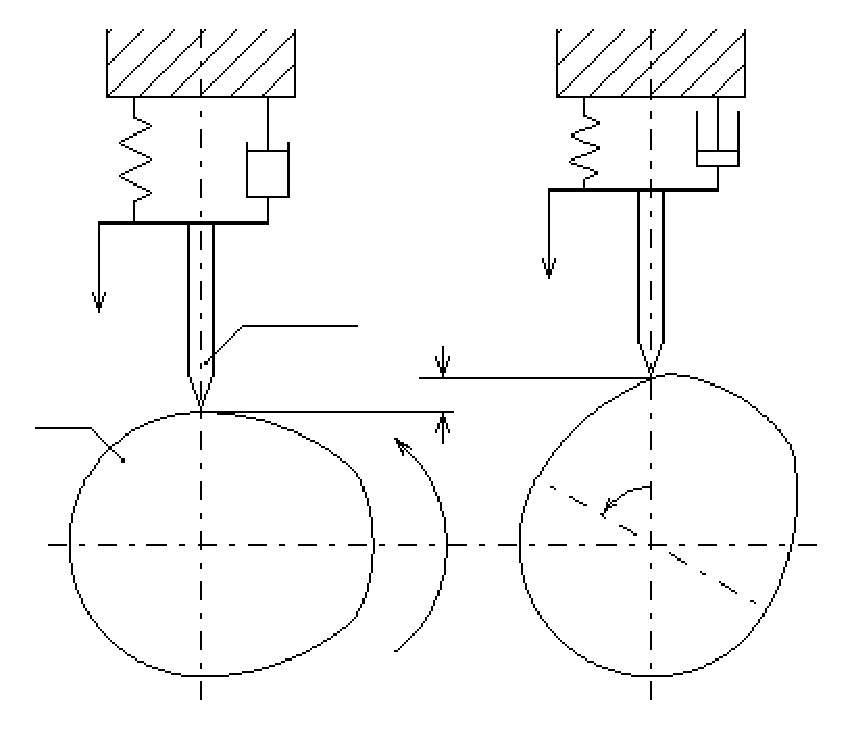
\includegraphics[height=8cm]{./Figures/cam}}}
 \put (0,52){\mbox{$F_{v}$}}
 \put (2,34.5){\mbox{\textit{Cam}}}
 \put (26,46){\mbox{\textit{Follower}}}
 \put (15,46){\mbox{\textit{$\mu$}}}
 \put (9,62){\mbox{$\kappa$}}
 \put (32,62){\mbox{$\zeta$}}
 \put (38,40){\mbox{$\delta c (\beta)$}}
 \put (66,28){\mbox{$\beta$}}
 \put (2.5,6){\mbox{\textit{$t=0$}}}
 \put (52.4,6){\mbox{\textit{$t=\beta$}}}
 \put (18.5,-1){\mbox{\textit{(a)}}}
 \put (69.4,-1){\mbox{\textit{(b)}}}
\end{picture}
\begin{picture}(90,80)(-3,0)
 \put (0,0){\mbox{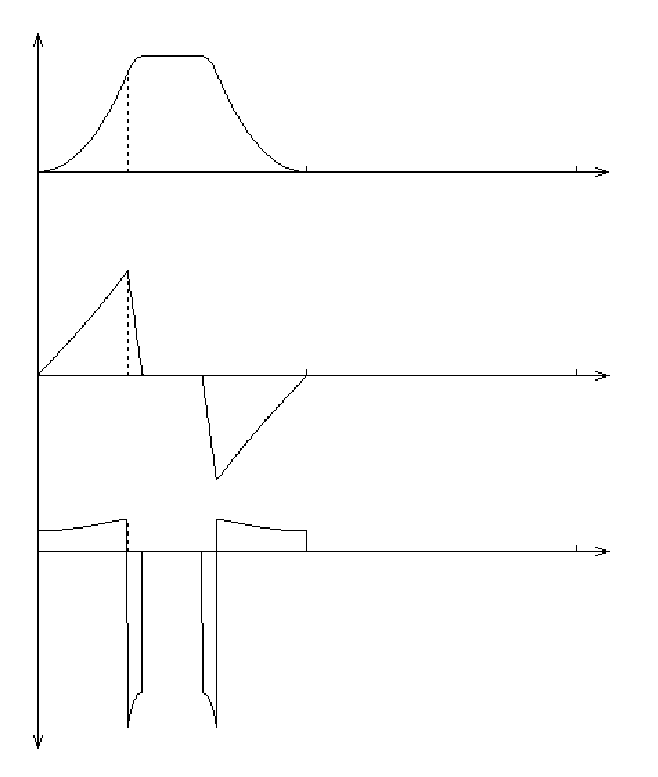
\includegraphics[height=8cm]{./Figures/campva}}}
 \put (-3,75){\mbox{$\delta c$}}
 \put (-3,49){\mbox{$ \frac{dc}{dt}$}}
 \put (-3,25){\mbox{$ \frac{d^2c}{dt^2}$}}
 \put (30,60){\mbox{$\pi$}} \put (58,60){\mbox{$2\pi$}}
 \put (10,60){\mbox{$\beta$}}
% \put (30,38){\mbox{$\pi$}} \put (58,38){\mbox{$2\pi$}}
% \put (9,38){\mbox{$\beta$}}
% \put (30,19){\mbox{$\pi$}} \put (58,19){\mbox{$2\pi$}}
% \put (9,19){\mbox{$\beta$}}
 \put (32,-1){\mbox{\textit{(c)}}}
\end{picture}
%\begin{picture}(45,20)(-90,-20)
% \put (3,10){\mbox{$v^{+}=(1+r)\frac{dc}{dt}-rv^{-}$}}
% \put (16,-1){\mbox{\textit{(d)}}}
%\end{picture}
%\begin{picture}(45,20)(-85,-20)
% \put (-2,20){\mbox{$k \hspace{4mm}= \hspace{1.5mm}5 \times 10^{4}\hspace{1.5mm} (N /m)$}}
% \put (-2,16){\mbox{$b \hspace{4mm}= \hspace{1.5mm}0 \hspace{10.5mm}(N\hspace{0.5mm} s/m)$}}
% \put (-2,12){\mbox{$F_{ext} \hspace{0.2mm}= \hspace{1.5mm}0 \hspace{12.5mm}(N)$}}
% \put (-2,8){\mbox{$c \hspace{4mm}\in \hspace{1.5mm}[0.52\hspace{2mm} 0.67]\hspace{2mm}(m)$}}
% \put (-2,4){\mbox{$r \hspace{4mm}= \hspace{1.5mm}0.9$}}
% \put (16,-1){\mbox{\textit{(e)}}}
%\end{picture}
  \caption{Cam-Shaft's schematics. \textit{(a)} t=0. \textit{(b)} t=$\beta$. \textit{(c)} Constraint position $\delta c(t)$, velocity $\frac{dc}{dt}(t)$ and acceleration $\frac{d^{2}c}{dt}(t^{2})$.}
  \label{Fig:cam-shaft}
\end{figure}
\subsection{The cam-follower as a Lagrangian NSDS.}
%\textit{\textbf{WP2 Template 1 Simulation of a bouncing ball with the Moreau's Time-Stepping scheme.}\\{Acary}}\\
 It is possible to completely describe the cam-follower system as a
 driven impact oscillator into the framework of \textit{Lagrangian NSDS} using a
translation in space. Setting $\hat u(t)=u(t)-c(t)$ and $\hat
v(t)= v(t)-dc/dt$, then equations (\ref{eq:sols}) and
(\ref{eq:il}) can be expressed as (the argument $t$ will not be
explicitly written)
\begin{eqnarray}
  \label{eq:trans}
  \mu\frac{d^2\hat u}{dt^2}+\zeta\frac{d\hat u}{dt}+\kappa
  \hat u=f_{v}-\left(\mu\frac{d^2c}{dt^2}+\zeta\frac{dc}{dt}+\kappa
  c\right)&\equiv &\hat f,  \; \text{\hspace{6.5mm} \text{if} \hspace{3mm}$\hat u >
 0$.}\\
\hat v^+&=&-r \hat v^- , \; \text{ \text{if}\hspace{3mm}$\hat
u=0$.}
\end{eqnarray}
Using the framework presented in [2] we have that the equation of
motion of a Lagrangian system may be stated as follows :
\begin{eqnarray}
  \label{eq:lag1}
  M(q)\ddot q + Q(q,\dot q) + F(\dot q, q , t) = F_{ext}(t) + R
\end{eqnarray}

From the (\ref{eq:trans}) we can derive all of the terms which
define a Lagrangian NSDS. In our case the model is completely
linear:
\begin{eqnarray}
  \nonumber
  q&=& \left[\begin{array}{c}  \hat u  \end{array}\right]    \\
  \nonumber
  M(q)&=&  \left[\begin{array}{c} \mu  \end{array}\right] \\
  \label{eq:lag2}
  Q(q,\dot q )& = &\left[\begin{array}{c} 0  \end{array}\right]  \\
  \nonumber
  F(q, \dot q ) &=&  \left[\begin{array}{c} \zeta \end{array}\right] \dot q +  \left[\begin{array}{c} \kappa  \end{array}\right] q\\
  \nonumber
  F_{ext}& = & \left[\begin{array}{c} \hat f \end{array}\right]
\end{eqnarray}

The unilateral constraint requires that:
\begin{eqnarray}
\label{eq:constr} \nonumber
 \hat u \geq 0
\end{eqnarray}
so we can obtain
\begin{eqnarray}
y &= & H^T q + b \\
\nonumber H^T &=&\left[\begin{array}{c} 1 \end{array}\right]\\
\nonumber b&=&0
\end{eqnarray}

In the same way, the reaction force due to the constraint is
written as follows:
\begin{eqnarray}
\nonumber R=H \lambda, \hspace{1cm}  \text{with }
H=\left[\begin{array}{c} 1
\end{array}\right]
\end{eqnarray}

The unilataral contact law may be formulated as follow:
\begin{eqnarray}
  \label{eq:119}
  0 \leq y \perp \lambda\geq 0
\end{eqnarray}
and the Newton's impact law:
\begin{eqnarray}
  \label{eq:120}
\text{If } y=0, \dot{y}^+ =-r\dot{y}^-
\end{eqnarray}

\subsection{Implementation in the platform}
%The code for the simulation of the Cam Follower system using the
%SICONOS software package is:
For the simulation of the cam follower system follow the steps

\begin{enumerate}
\item Move to the working directory \verb"sample/CamFollower"

\verb"$cd sample/CamFollower "

\item Clean the directory form binary files using the
\verb"siconos" command

\verb"$siconos -c "

\item Compile the file \verb"CamFollowerNoXml.cpp" in
the sample folder ({\em See} the code at the end of the section)

\verb"$siconos CamFollowerNoXml.cpp"

\item Change the simulation parameters ({\em i.e.}
Follower initial position and velocity, cam initial angle,
simulations time, cam rotational speed in rpm, etc.) in the file
\verb"CamFollowerNoXml.cpp".

\end{enumerate}

Next we present the sample code for the
\verb"CamFollowerNoXml.cpp" file:
\begin{tabbing}
\hspace{1cm}\= \hspace{0.5cm}\= \hspace{1cm}\= \hspace{1cm}\= \hspace{1cm}\\
 \> \+ int main(int argc, char* argv[]) {\bf \{} \\
 \>  {\bf\{} \+ \hspace{0.5cm}\= \hspace{2cm}\= \hspace{1cm}\=\hspace{1cm}\=\hspace{1cm}\=\hspace{1cm}\=\\
 \> \em   // ======== Creation of the model =============\\
 \> \em  // User-defined main parameters\\

 \> double rpm=358; \\
 \> double phi\_0=0;\\

 \> unsigned int dsNumber = 1; \>\>\>\> \em // the Follower and the ground\\
 \> unsigned int nDof = 1;  \>\>\>\>    \em // degrees of freedom for the Follower\\
 \> double t0 = 0;            \>\>\>\>  \em   // initial computation time\\
 \> double T = 5;             \>\>\>\>  \em    // final computation time\\
 \> double h = 0.0001;   \>\>\>\>       \em // time step\\
 \> int Kplot;\\
 \> Kplot=(int)(Tplot/h);\\

 \> double position\_init = 0.4;\>\>\>\> \em// initial position for lowest bead.\\
 \> double velocity\_init = 0.4;\>\>\>\> \em// initial velocity for lowest bead.\\
 \\
 \> \em    // ======= Dynamical systems =========\\
 \\
 \>     vector<DynamicalSystem *> vectorDS; // the list of DS\\
 \>     vectorDS.resize(dsNumber,NULL);\\
\\
 \> SiconosMatrix *Mass, *K, *C;        // mass/rigidity/viscosity\\
 \> Mass = new SiconosMatrix(nDof,nDof);\\
 \> (*Mass)(0,0) = 1.221;\\
 \> K = new SiconosMatrix(nDof,nDof);\\
 \> (*K)(0,0) = 1430.8;\\
 \> C = new SiconosMatrix(nDof,nDof);\\
 \> (*C)(0,0) = 0;\\
\\
 \>  //  Initial positions and velocities  \\
 \>  vector<SimpleVector *> position\_0;\\
 \>  vector<SimpleVector *> velocity\_0;\\
 \>  position\_0.resize(dsNumber,NULL);\\
 \>  velocity\_0.resize(dsNumber,NULL);\\
 \>  position\_0[0] = new SimpleVector(nDof);\\
 \>  velocity\_0[0] = new SimpleVector(nDof);\\
 \>  (*(position\_0[0]))(0) = position\_init;\\
 \>  (*(velocity\_0[0]))(0) = velocity\_init;\\
 \\
 \>  vectorDS[0] =\\ \>
 new LagrangianLinearTIDS(0,nDof,*(position\_0[0]),*(velocity\_0[0]),*Mass,*K,*C);\\
\\
 \> static\_cast<LagrangianDS*>(vectorDS[0])
 \\ \>\>\>->setComputeFExtFunction("FollowerPlugin.so", "FollowerFExt");\\
\\
 \> // Example to set a list of parameters in FExt function.\\
 \> // 1 - Create a simple vector that contains the required
 parameters.\\
\\
 \> // Here we set two parameters, the DS  number.\\
 \> SimpleVector * param = new SimpleVector(2);\\
\\
 \> (*param)(0)=rpm;\\
 \> (*param)(1)=phi\_0;\\
 \> // 2 - Assign this param to the function FExt\\
 \> static\_cast<LagrangianDS*>(vectorDS[0])->setParametersListPtr(param,2);\\
 \> // 2 corresponds to the position of FExt in the stl vector of possible parameters. \\
\> //  0 is mass, 1 FInt.\\ % and so on.\\
 \> // Now the cam rotational velocity in rpms will be available in FExt plugin.\\
\\
\> // ===== Interactions =====\\
\\
 \>  vector<Interaction*> interactionVector;\\
 \>  interactionVector.resize(1,NULL);\\
 \>  vector<DynamicalSystem*> *dsConcerned = \\ \>\>\> new vector<DynamicalSystem*>(dsNumber);\\
\\
 \>  // ===== Non Smooth Law =====\\
 \>  double e = 0.8;\\

 \>  // Interaction Follower-floor\\
 \>  SiconosMatrix *H = new SiconosMatrix(1,nDof);\\
 \>  (*H)(0,0) = 1.0;\\
 \>  NonSmoothLaw * nslaw = new NewtonImpactLawNSL(e);\\
 \>  Relation * relation = new LagrangianLinearR(*H);\\
 \>  (*dsConcerned)[0] = vectorDS[0];\\

 \>  interactionVector[0] = new Interaction("Follower-Ground",0,1, dsConcerned);\\
 \>  interactionVector[0]->setRelationPtr(relation);\\
 \>  interactionVector[0]->setNonSmoothLawPtr(nslaw);\\

 \> // ===== Interactions =====\\
\\
 \> // ===== NonSmoothDynamicalSystem =====\\

 \> bool isBVP =0;\\
 \> NonSmoothDynamicalSystem * nsds = \\
\>\>\>\> new NonSmoothDynamicalSystem(isBVP);\\
\\
 \>// Set DS of this NonSmoothDynamicalSystem\\
 \> nsds->setDynamicalSystems(vectorDS);       \\
 \> // Set interactions of the  NonSmoothDynamicalSystem\\
 \> nsds->setInteractions(interactionVector);  \\
\\
 \> // ===== Model =====\\
\\
 \> Model * Follower = new Model(t0,T);\\
 \> // set NonSmoothDynamicalSystem of this  model\\
 \> Follower->setNonSmoothDynamicalSystemPtr(nsds);\\
 \\
 \> // ====== Strategy ======\\
\\
 \> double theta = 0.5;  \>\>\>      // theta for Moreau integrator\\
 \> string solverName = "QP" ;\\
\\
 \> Strategy* S = new TimeStepping(Follower);\\
\\
 \> // -- Time discretisation --\\
 \> TimeDiscretisation * t = new TimeDiscretisation(h,S);\\
\\
 \> // -- OneStepIntegrators --\\
 \> vector<OneStepIntegrator *> vOSI;\\
 \> vOSI.resize(dsNumber,NULL);\\
 \> vOSI[0] = new Moreau(t,vectorDS[0],theta);\\
 \> S->setOneStepIntegrators(vOSI);\\
\\
 \> // -- OneStepNsProblem --\\
 \> OneStepNSProblem * osnspb = new LCP(S,solverName,101, 0.0001,"max",0.6);\\
 \> S->setOneStepNSProblemPtr(osnspb); // set OneStepNSProblem of the
 strategy\\
 \> cout << "=== End of model loading === " << endl;\\
 \> // ==== End of model definition======\\
\\
\\
\\
 \> // ========= Computation============\\
\\
 \> // --- Strategy initialization ---\\
 \> S->initialize();\\
 \> cout <<"End of strategy initialisation" << endl;\\
\\

 \> int k = t->getK(); \> \> \> \> // Current step\\
 \> int N = t->getNSteps(); \> \> \> \> // Number of time steps\\
\\
 \> // --- Get the values to be plotted ---\\
 \> // -> saved in a matrix dataPlot\\
 \> unsigned int outputSize = 8;\\
\\
 \> SiconosMatrix DataPlot(Kplot+1,outputSize );\\
 \>   // For the initial time step:\\
 \\
 \> // time\\
 \>     DataPlot(k,0) = k*t->getH();\\
 \\
 \>     DataPlot(k,1) = static\_cast<LagrangianDS*>(vectorDS[0])->getQ()(0);\\
 \>     DataPlot(k,2) = static\_cast<LagrangianDS*>(vectorDS[0])->getVelocity()(0);\\
 \>     DataPlot(k,3) = (Follower->getNonSmoothDynamicalSystemPtr()->\\
 \> \> getInteractionPtr(0)->getLambda(1))(0);\\
 \>     DataPlot(k,4) = static\_cast<LagrangianDS*>(vectorDS[0])->getFExt()(0);\\
 \\
 \>     // State of the Cam\\
 \>      double CamEqForce,CamPosition,CamVelocity,CamAcceleration;\\

 \>     CamEqForce=\\
 \> \> CamState(k*t->getH(),rpm,CamPosition,CamVelocity,CamAcceleration);\\
 \>     // Position of the Cam\\
 \>      DataPlot(k, 5) = CamPosition;\\
 \>      // Velocity of the Cam\\
 \>      DataPlot(k, 6) = CamVelocity;\\
 \>      // Acceleration of the Cam\\
 \>      DataPlot(k, 7) =\\
 \> \>CamPosition+static\_cast<LagrangianDS*>(vectorDS[0])->getQ()(0);\\
\\
 \> // --- Time loop ---\\
 \> cout << "Start computation ... " << endl;\\
 \> while(k < N)\\
 \>   {\bf \{ }\+ \hspace{0.5cm}\= \hspace{2cm}\= \hspace{1cm}\=\hspace{1cm}\=\hspace{1cm}\=\hspace{1cm}\=\\\\
 \> // --- Get values to be plotted ---\\
 \>     DataPlot(k,0) = k*t->getH();\\
 \\
 \>     DataPlot(k,1) = \\
 \> \> static\_cast<LagrangianDS*>(vectorDS[0])->getQ()(0);\\
 \>     DataPlot(k,2) =  \\
 \> \> static\_cast<LagrangianDS*>(vectorDS[0])->getVelocity()(0);\\
 \>     DataPlot(k,3) =  \\
 \> \> (Follower->getNonSmoothDynamicalSystemPtr()->\\
 \> \> getInteractionPtr(0)->getLambda(1))(0);\\
 \>     DataPlot(k,4) = static\_cast<LagrangianDS*>(vectorDS[0])->getFExt()(0);\\
 \\

 \>     CamEqForce=\\
 \>  CamState(k*t->getH(),rpm,CamPosition,CamVelocity,CamAcceleration);\\
 \\
 \>      DataPlot(k, 5) = CamPosition;\\
 \>      DataPlot(k, 6) = CamVelocity;\\
 \>      DataPlot(k, 7) = CamPosition+\\
 \> \> static\_cast<LagrangianDS*>(vectorDS[0])->getQ()(0);\\

 \> // transfer of state i+1 into state i and time
 incrementation\\
 \> S->nextStep();\\

 \> // get current time step\\
 \> k = t->getK();\\
 \> // solve ...\\
 \> S->computeFreeState();\\
 \> S->computeOneStepNSProblem();\\
 \> // update\\
 \> S->update();
 \-\\
 \>   {\bf \} }\\
\>    // --- Output files ---\\
 \> DataPlot.rawWrite("result.dat", "ascii");\\

 \> // --- Free memory ---\\
 \> delete osnspb;\\
 \> delete vOSI[0];\\
 \> delete t;\\
 \> delete S;\\
 \> delete Follower;\\
 \> delete nsds;\\
 \> delete interactionVector[0];\\
 \> delete relation;\\
 \> delete nslaw;\\
 \> delete H;\\
 \> delete dsConcerned;\\
 \> delete vectorDS[0];\\
 \> delete position\_0[0];\\
 \> delete velocity\_0[0];\\
 \> delete C;\\
 \> delete K;\\
 \> delete Mass;\\

    \-\\
 \>  {\bf\}}
\end{tabbing}
%\end{enumerate}
\newpage
\subsection{Simulation}
We have perform the simulation of the cam follower system for
different values of the cam rotational speed with the SICONOS
software package using a time-stepping numerical scheme with step
size ($h=1e^{-4}$) and an event-driven scheme with minimum step
size \linebreak ($h_{min}=1e^{-12}$). Fig.
\ref{Fig:time_comparison} and \ref{Fig:state_comparison} show the
time simulations for different values of the cam rotational speed
and Fig. \ref{Fig:attractor_comparison} show the chaotic attractor
at $rpm=660$ for impact and stroboscopic Poincar\`e sections.

\begin{figure}[hbtp]
\vspace{5mm} \setlength{\unitlength}{1mm}
\begin{picture}(60,60)(0,-7)
 \put (0,0){\mbox{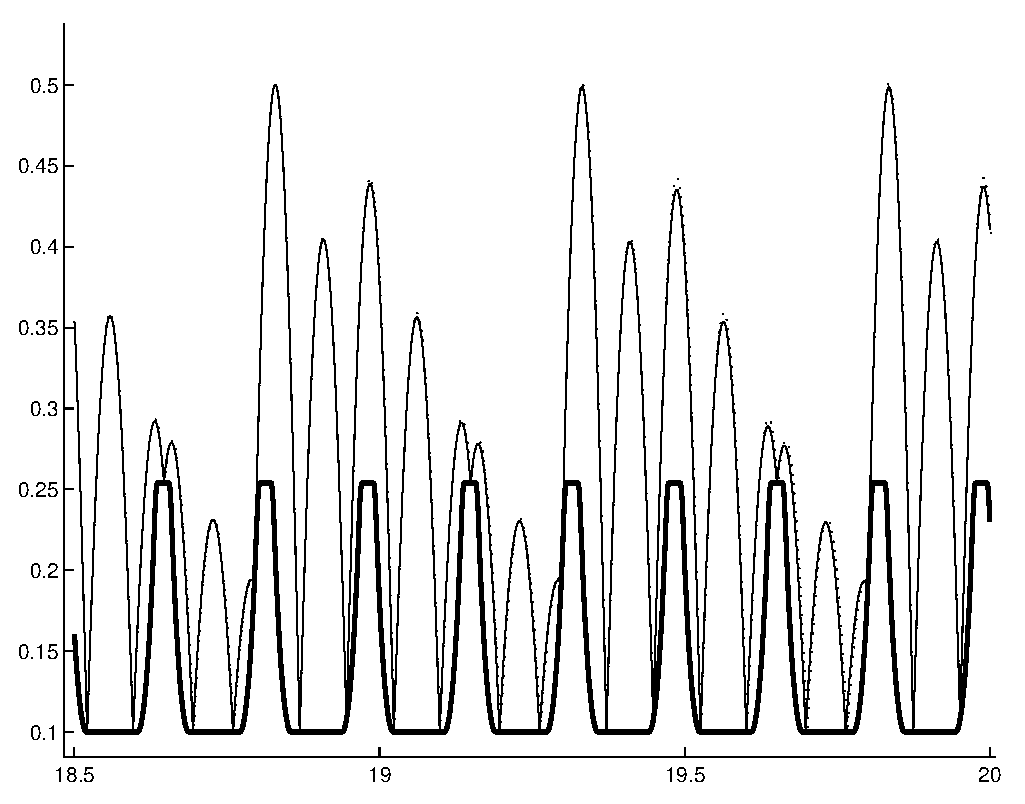
\includegraphics[height=6cm]{./comparison_figs/time_comparison_358}}}
  \put (35,-4){\mbox{\textit{(a)}}}
\end{picture}
\begin{picture}(60,60)(15,-7)
 \put (0,0){\mbox{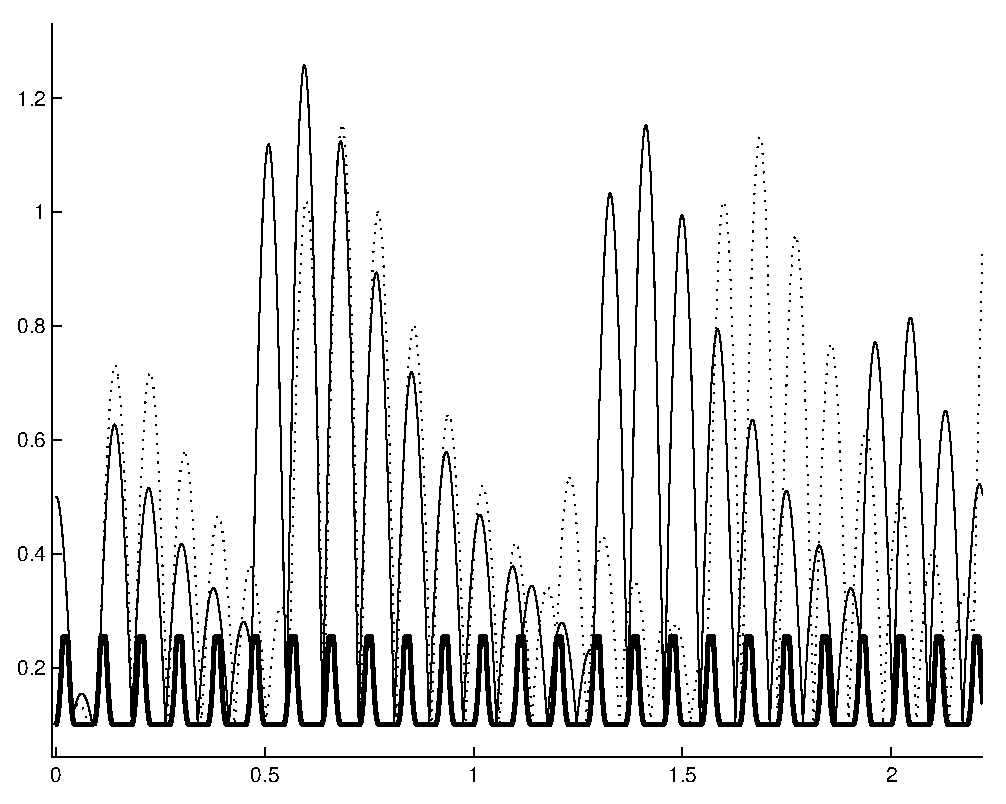
\includegraphics[height=6cm]{./comparison_figs/time_comparison_660}}}
 \put (35,-4){\mbox{\textit{(b)}}}
\end{picture}
\begin{picture}(60,60)(-40,-2)
 \put (0,0){\mbox{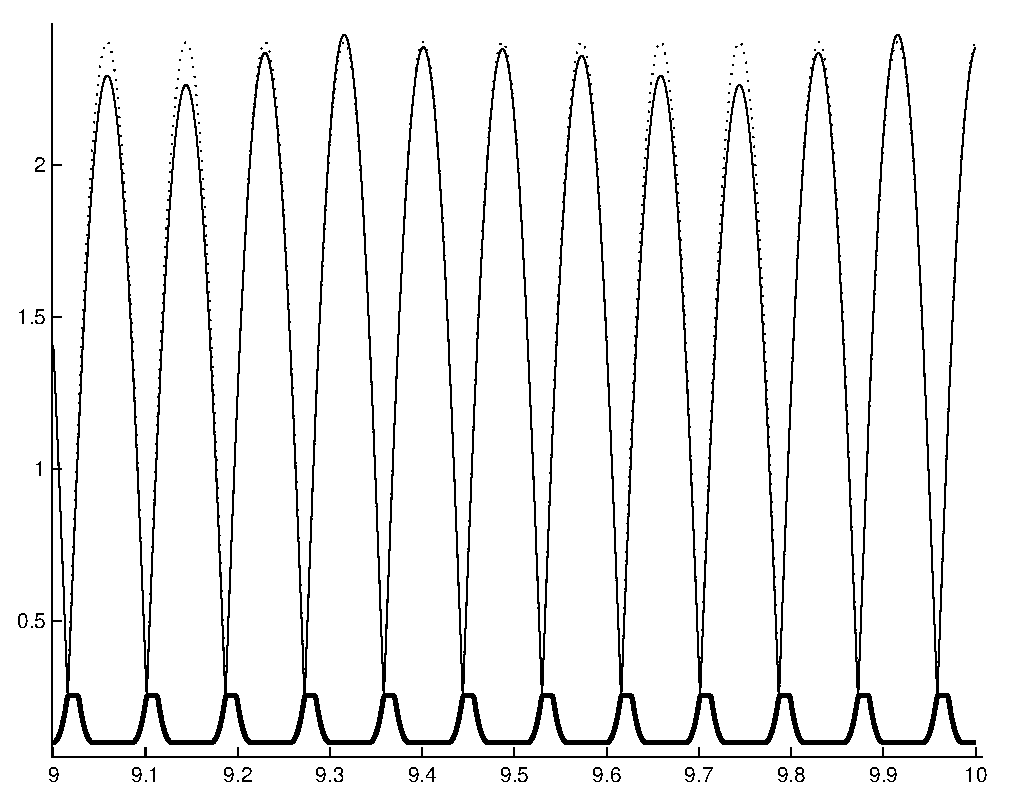
\includegraphics[height=6cm]{./comparison_figs/time_comparison_700}}}
 \put (35,-4){\mbox{\textit{(c)}}}
\end{picture}
  \caption{Time series using SICONOS platform. Time-stepping scheme (continuous line). Event-driven scheme (dashed line) \textit{(a)} rpm=358. \textit{(b)} rpm=660. \textit{(c)} rpm=700.}
  \label{Fig:time_comparison}
\end{figure}

\begin{figure}[hbtp]
\vspace{5mm} \setlength{\unitlength}{1mm}
\begin{picture}(60,60)(0,-7)
 \put (0,0){\mbox{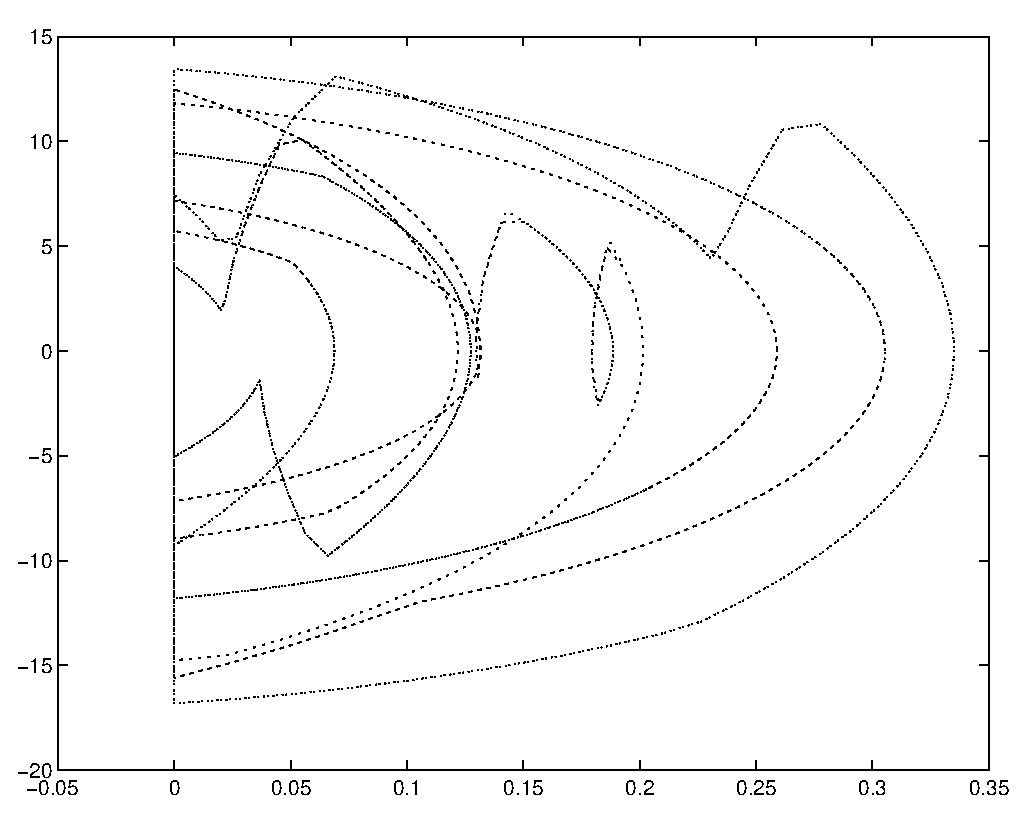
\includegraphics[height=6cm]{./comparison_figs/state_comparison_358event}}}
  \put (35,-4){\mbox{\textit{(a)}}}
\end{picture}
\begin{picture}(60,60)(15,-7)
 \put (0,0){\mbox{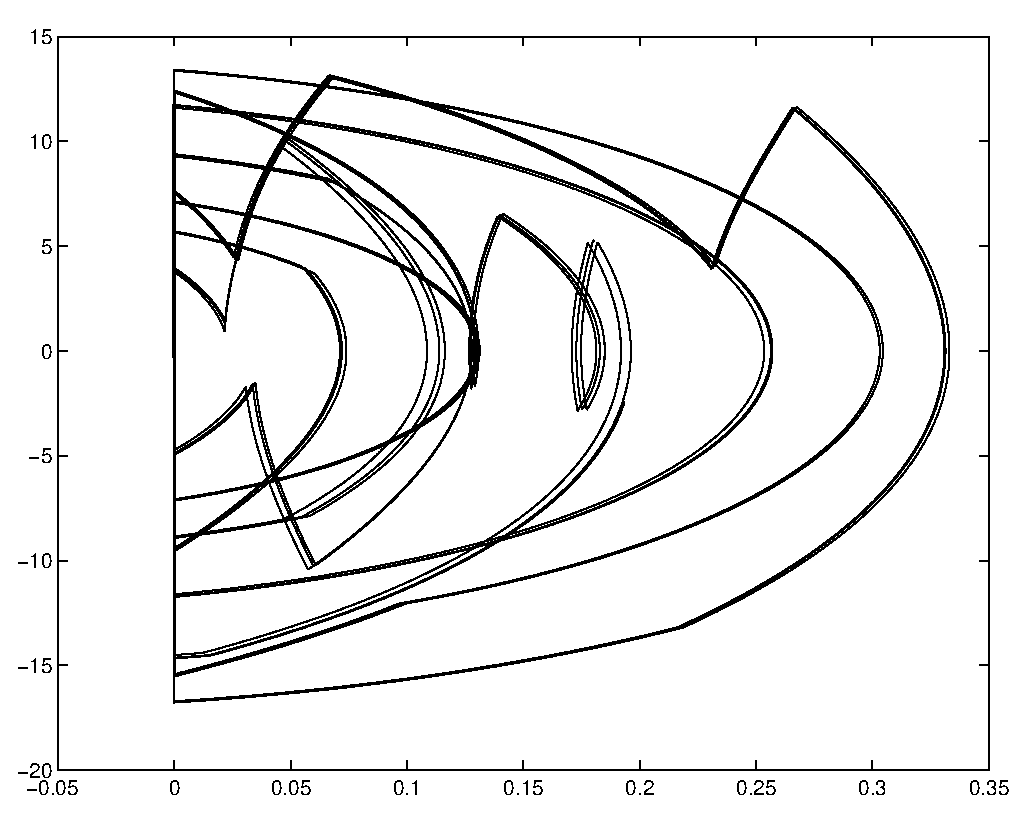
\includegraphics[height=6cm]{./comparison_figs/state_comparison_358siconos}}}
 \put (35,-4){\mbox{\textit{(b)}}}
\end{picture}
\begin{picture}(60,60)(0,-2)
 \put (0,0){\mbox{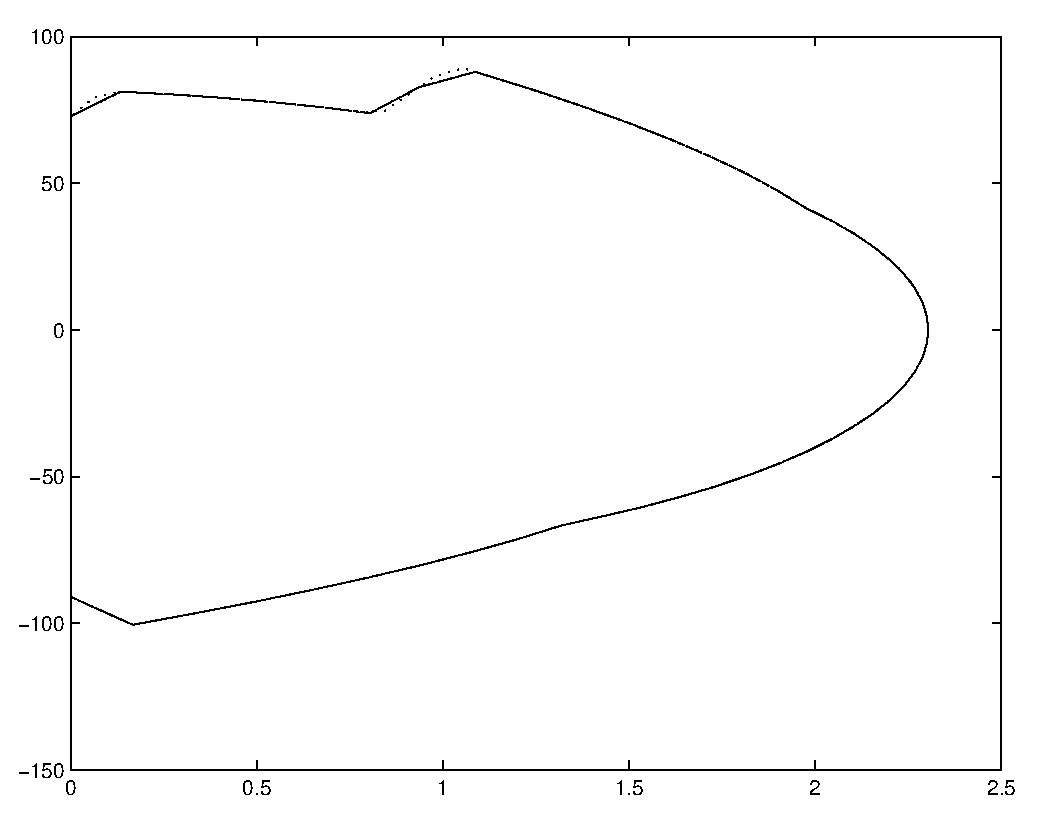
\includegraphics[height=6cm]{./comparison_figs/state_comparison_700event}}}
  \put (35,-4){\mbox{\textit{(c)}}}
\end{picture}
\begin{picture}(60,60)(-17,-2)
 \put (0,0){\mbox{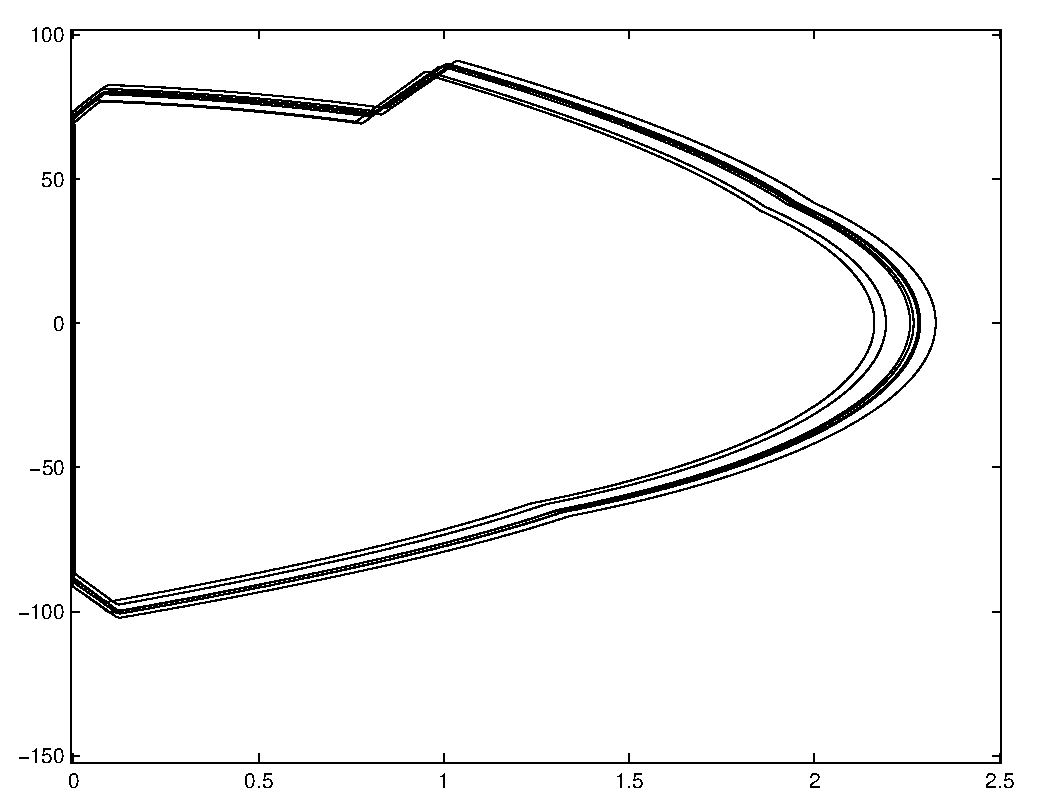
\includegraphics[height=6cm]{./comparison_figs/state_comparison_700siconos}}}
 \put (35,-4){\mbox{\textit{(d)}}}
\end{picture}
  \caption{State space comparison using SICONOS platform. \textit{(a)} rpm=358. Event Driven \textit{(b)} rpm=358. Time Stepping ($h=1e^{-4}$)\textit{(c)} rpm=700. Event Driven \textit{(d)} rpm=700. Time Stepping ($h=1e^{-4}$)}
  \label{Fig:state_comparison}
\end{figure}

\begin{figure}[hbtp]
\vspace{5mm} \setlength{\unitlength}{1mm}
\begin{picture}(60,60)(0,-7)
 \put (0,0){\mbox{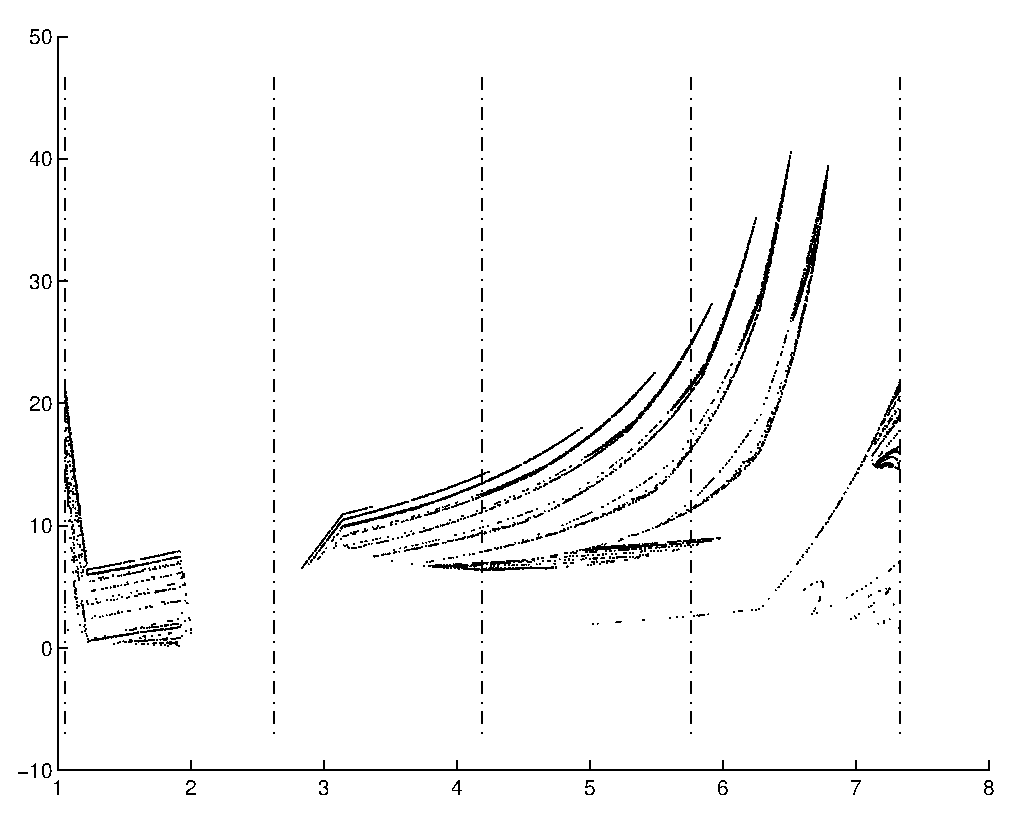
\includegraphics[height=6cm]{./comparison_figs/impact_map_660event}}}
  \put (35,-4){\mbox{\textit{(a)}}}
\end{picture}
\begin{picture}(60,60)(15,-7)
 \put (0,0){\mbox{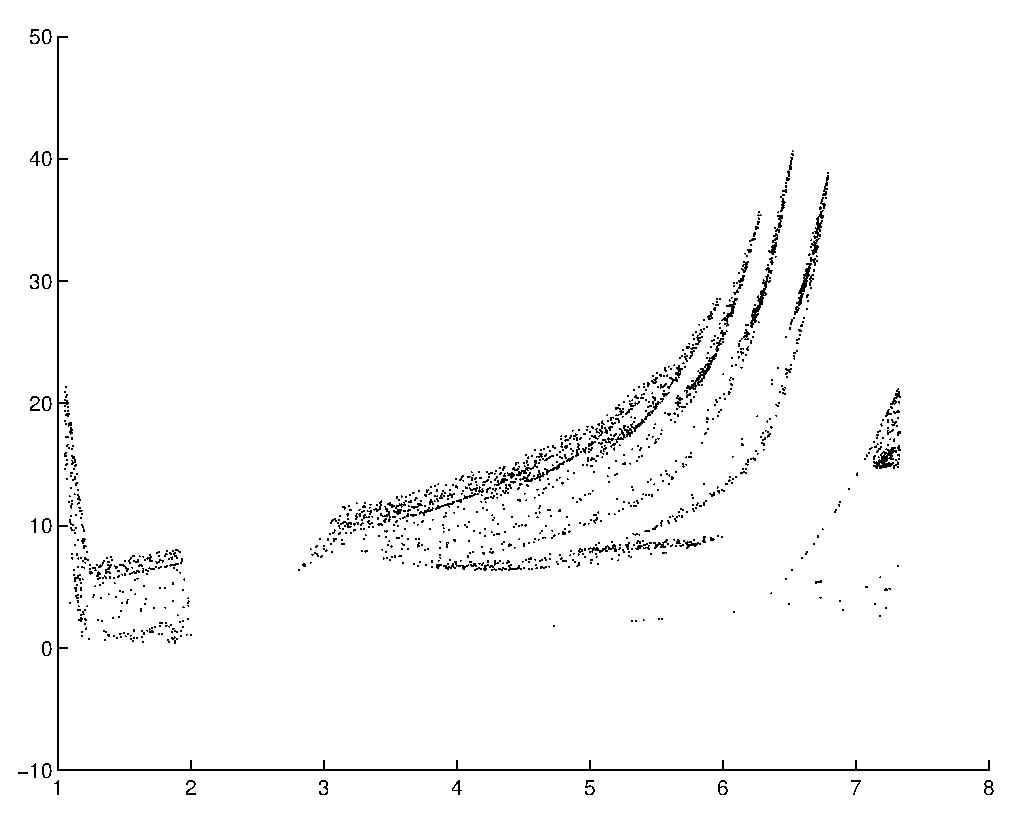
\includegraphics[height=6cm]{./comparison_figs/impact_map_660siconos}}}
 \put (35,-4){\mbox{\textit{(b)}}}
\end{picture}
\begin{picture}(60,60)(0,-2)
 \put (0,0){\mbox{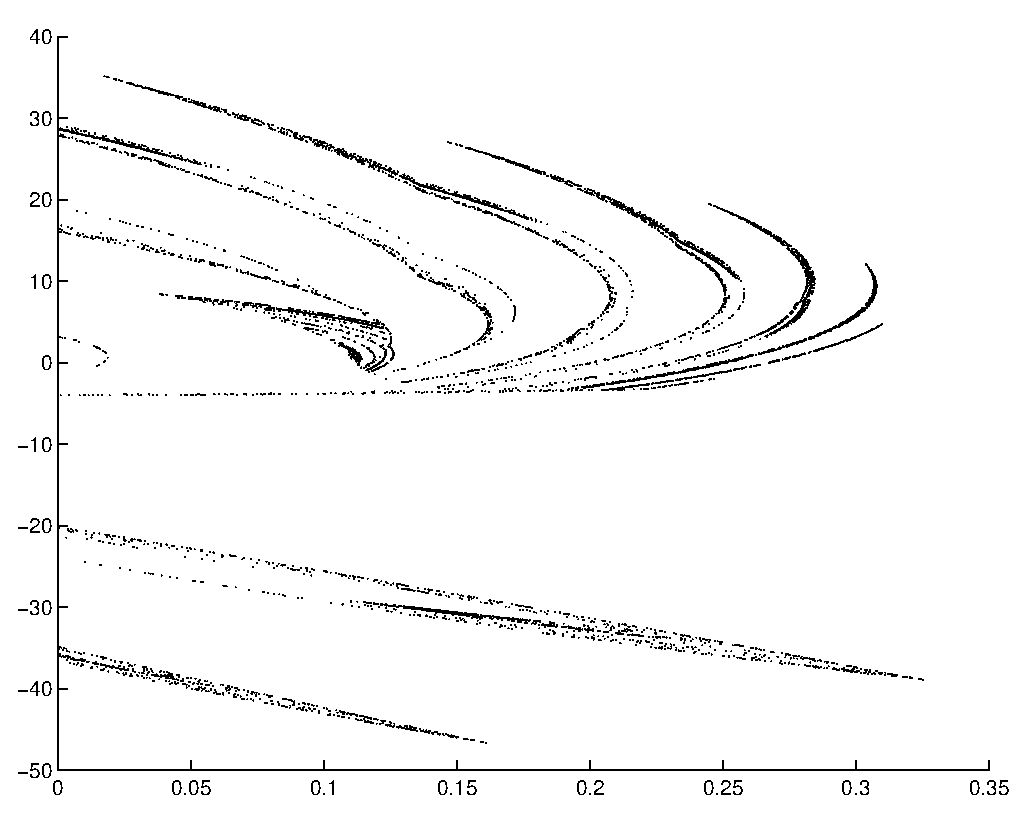
\includegraphics[height=6cm]{./comparison_figs/stroboscopic_map_660event}}}
  \put (35,-4){\mbox{\textit{(c)}}}
\end{picture}
\begin{picture}(60,60)(-17,-2)
 \put (0,0){\mbox{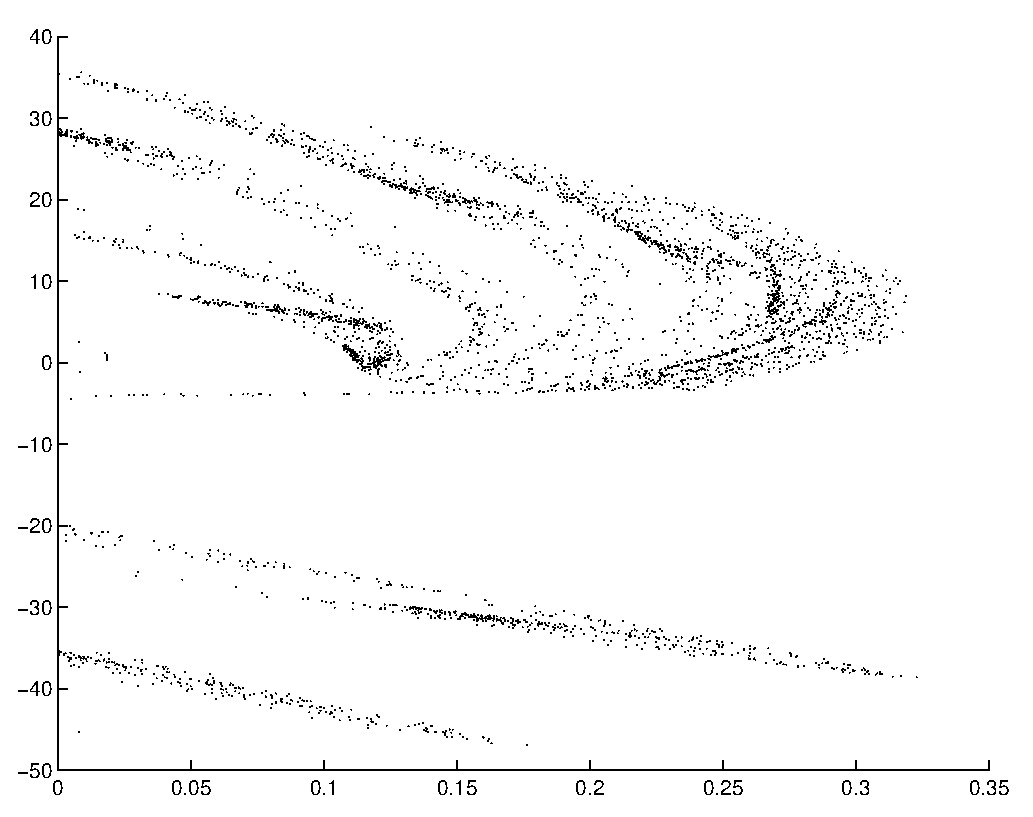
\includegraphics[height=6cm]{./comparison_figs/stroboscopic_map_660siconos}}}
 \put (35,-4){\mbox{\textit{(d)}}}
\end{picture}
  \caption{Attractors comparison using SICONOS platform at rpm=660. \textit{(a)}  Impact map. (Event Driven) \textit{(b)} Impact Map. Time Stepping ($h=1e^{-4}$)\textit{(a)}  Stroboscopic map. (Event Driven) \textit{(b)} Stroboscopic Map. Time Stepping ($h=1e^{-4}$)}
  \label{Fig:attractor_comparison}
\end{figure}
